\section{Cork Cancellations
} 
According to Post Office regulations, Postmasters were required to use ordinary letterstamps for defacing postage stamps on parcels. Damage often resulted as the hard face of the datestamp cut through the paper wrapping and to prevent this, postmasters and postal agents made their own personal dumb obliterators. Using cork or wood, they cut shapes and designs into the material. Such Cork obliterators (CO 1 to CO 13) were in use towards the turn of the last century and a large variety of them are noted. The use of these dumb obliterators was not authorised by the Postmaster General, but as they served the purpose so well officialdom not only turned a blind eye but also would appear to have actually encouraged their use.

\begin{figure*}
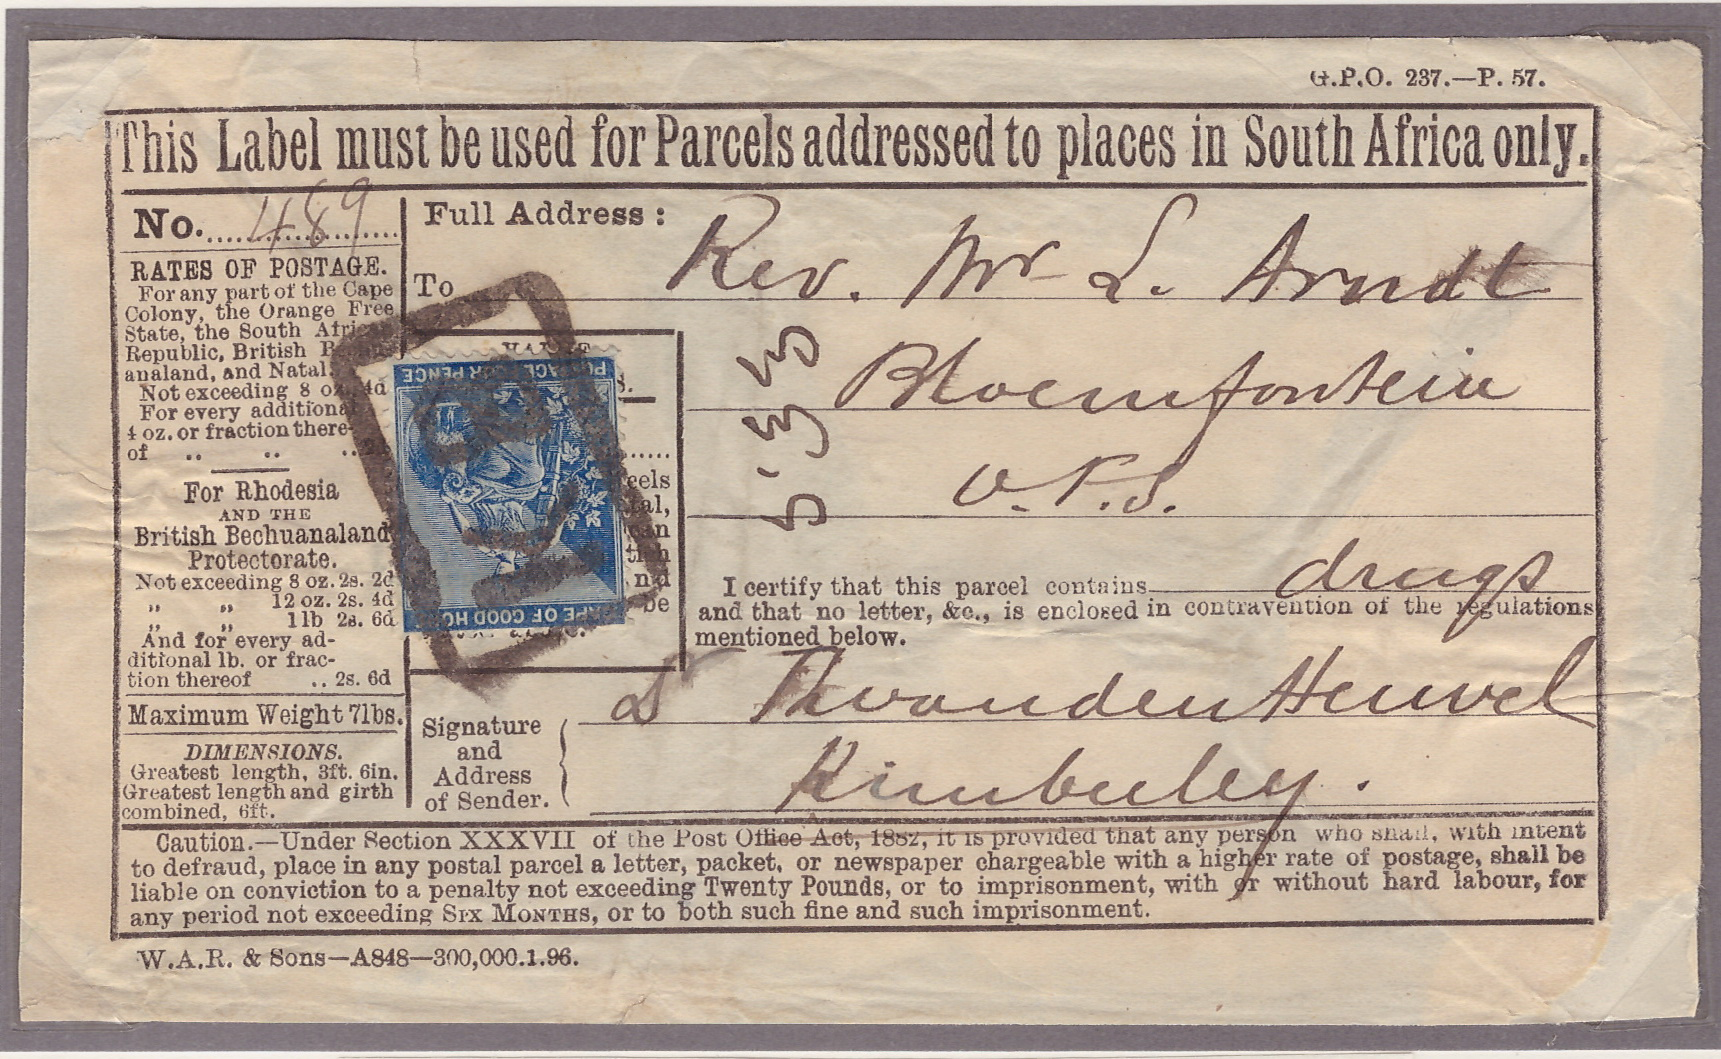
\includegraphics[width=1.0\textwidth]{../cape-of-good-hope/cork-kimberley.jpg}
\caption{A parcel post receipt stamped with a 4d blue Seated Hope obliterated with cork canceller with the letters "KB" for Kimberley.}
\end{figure*}


 

Simplicity of design was the keynote and most of the dumb cancellers are roughly cruciform, the cross being either in relief or sunken. Other commonly found designs include a series of bars, circles or squares.
	 
Many types are known and the illustrations and the study that follows here are by no means exhaustive.Stamps on covers are known to have been defaced with these Cork Obliterators, although this was unauthorised.

Only a few covers of this nature have been noted and they are rare. (One can also be never sure that the stamps were not forged).

\section{Cork cancellers that can be Identified}

 It is not easy to trace the origin of cork cancellations unless they are found on piece accompanied by a datestamp or the stamps must be on a piece or cover bearing some other form of marking that can assist to trace its origin. However, some are readily identifiable showing the initial of the town of origin. Thus there are "C" or "CT" for Cape Town, "EL" for East London, "P" for Paarl, "B" for Bedford and "HV" for Hanover, "KB" for Kimberley. A circular or square frame sometimes encloses initials.

\begin{figure}
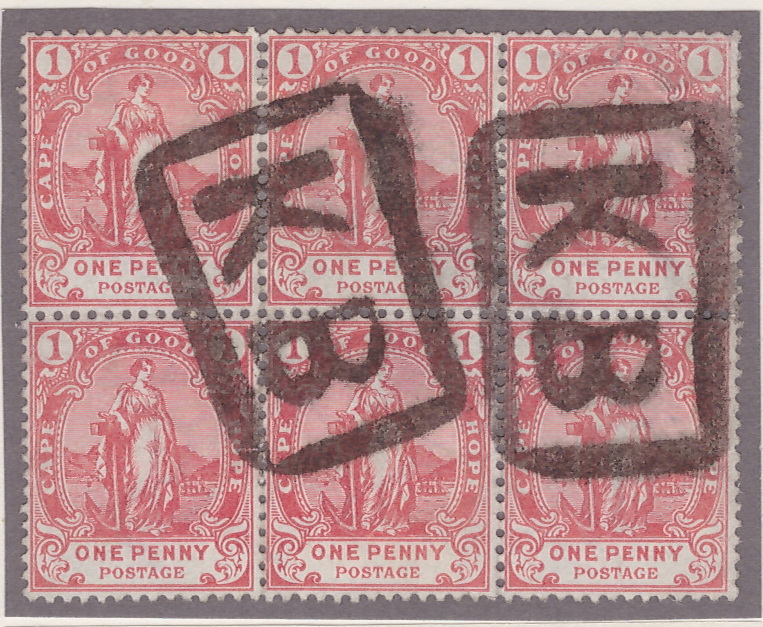
\includegraphics[width=1.0\textwidth]{../cape-of-good-hope/cork-kimberley-01.jpg}
\caption{Block of six with 1d red Standing Hope obliterated with rectangular cork canceller with the letters "KB" for Kimberley.}
\end{figure}

The cork parcel cancellers used in Cape Town are the easiest to identify as they bear the initial "C" or "CT". A number of distinct types can be identified. Figure~\ref{capecork01}
shows a circular cork obliterator with the letter "C" it is approximate 20mm in diameter and was probably carved from wood. The Postmaster tried to make it look similar to a Barred Oval Numeral Obliterator with two bar on the top and two at the bottom. 
\begin{marginfigure}
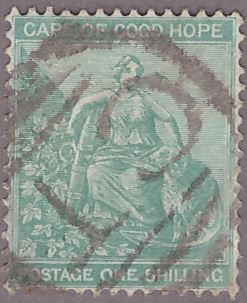
\includegraphics[width=1.0\textwidth]{../cape-of-good-hope/cork-cape-town-01.jpg}
\caption{Cape Town cork canceller.}
\label{capecork01}
\end{marginfigure}
If this was done to avoid any official criticism is unknown. This particular design is not very common probably due to the intricancy of the design and the ease that it could have been damaged.

\begin{figure}
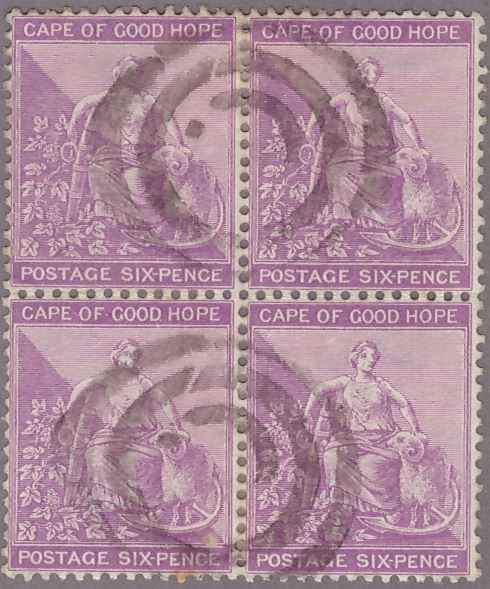
\includegraphics[width=0.6\textwidth]{../cape-of-good-hope/cork-cape-town.jpg}
\caption{Block of four with 6d lilac Seated Hope obliterated with circular cork canceller with the letter "C" for Cape Town.}
\end{figure}

Another interesting cork obliterator was that of Swellendam, which had the town name carved out as shown in Figure~\ref{swellendam}. 

\begin{figure}
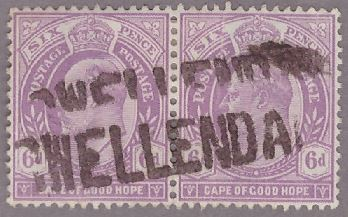
\includegraphics[width=0.6\textwidth]{../cape-of-good-hope/cork-swellendam.jpg}
\caption{Cork obliterator of Swellendam.}
\label{swellendam}
\end{figure}

A rare and probably unique cork canceller is that of Van der Blys Kraal. It consists of the place initials "VK" in large crude capital letters approximately 15mm height and 3mm thick, as shown in Figure~\ref{blyskraal}

\begin{figure}
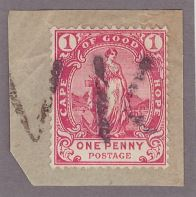
\includegraphics[width=0.35\textwidth]{../cape-of-good-hope/cork-blys.jpg}
\caption{Cork obliterator of van der Blys Kraal.}
\label{blyskraal}
\end{figure}

The Diamond Fields postmasters usually carved cancellers with a diamond shape and two distinct types have been identified so far.

\begin{figure}
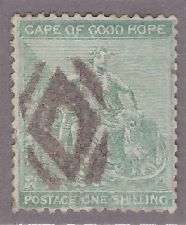
\includegraphics[width=0.35\textwidth]{../cape-of-good-hope/cork-diamond-fields.jpg}
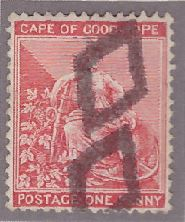
\includegraphics[width=0.35\textwidth]{../cape-of-good-hope/cork-diamond-fields-01.jpg}
\caption{Cork obliterators of Diamond Fields.}
\label{blyskraal}
\end{figure}





\begin{figure*}
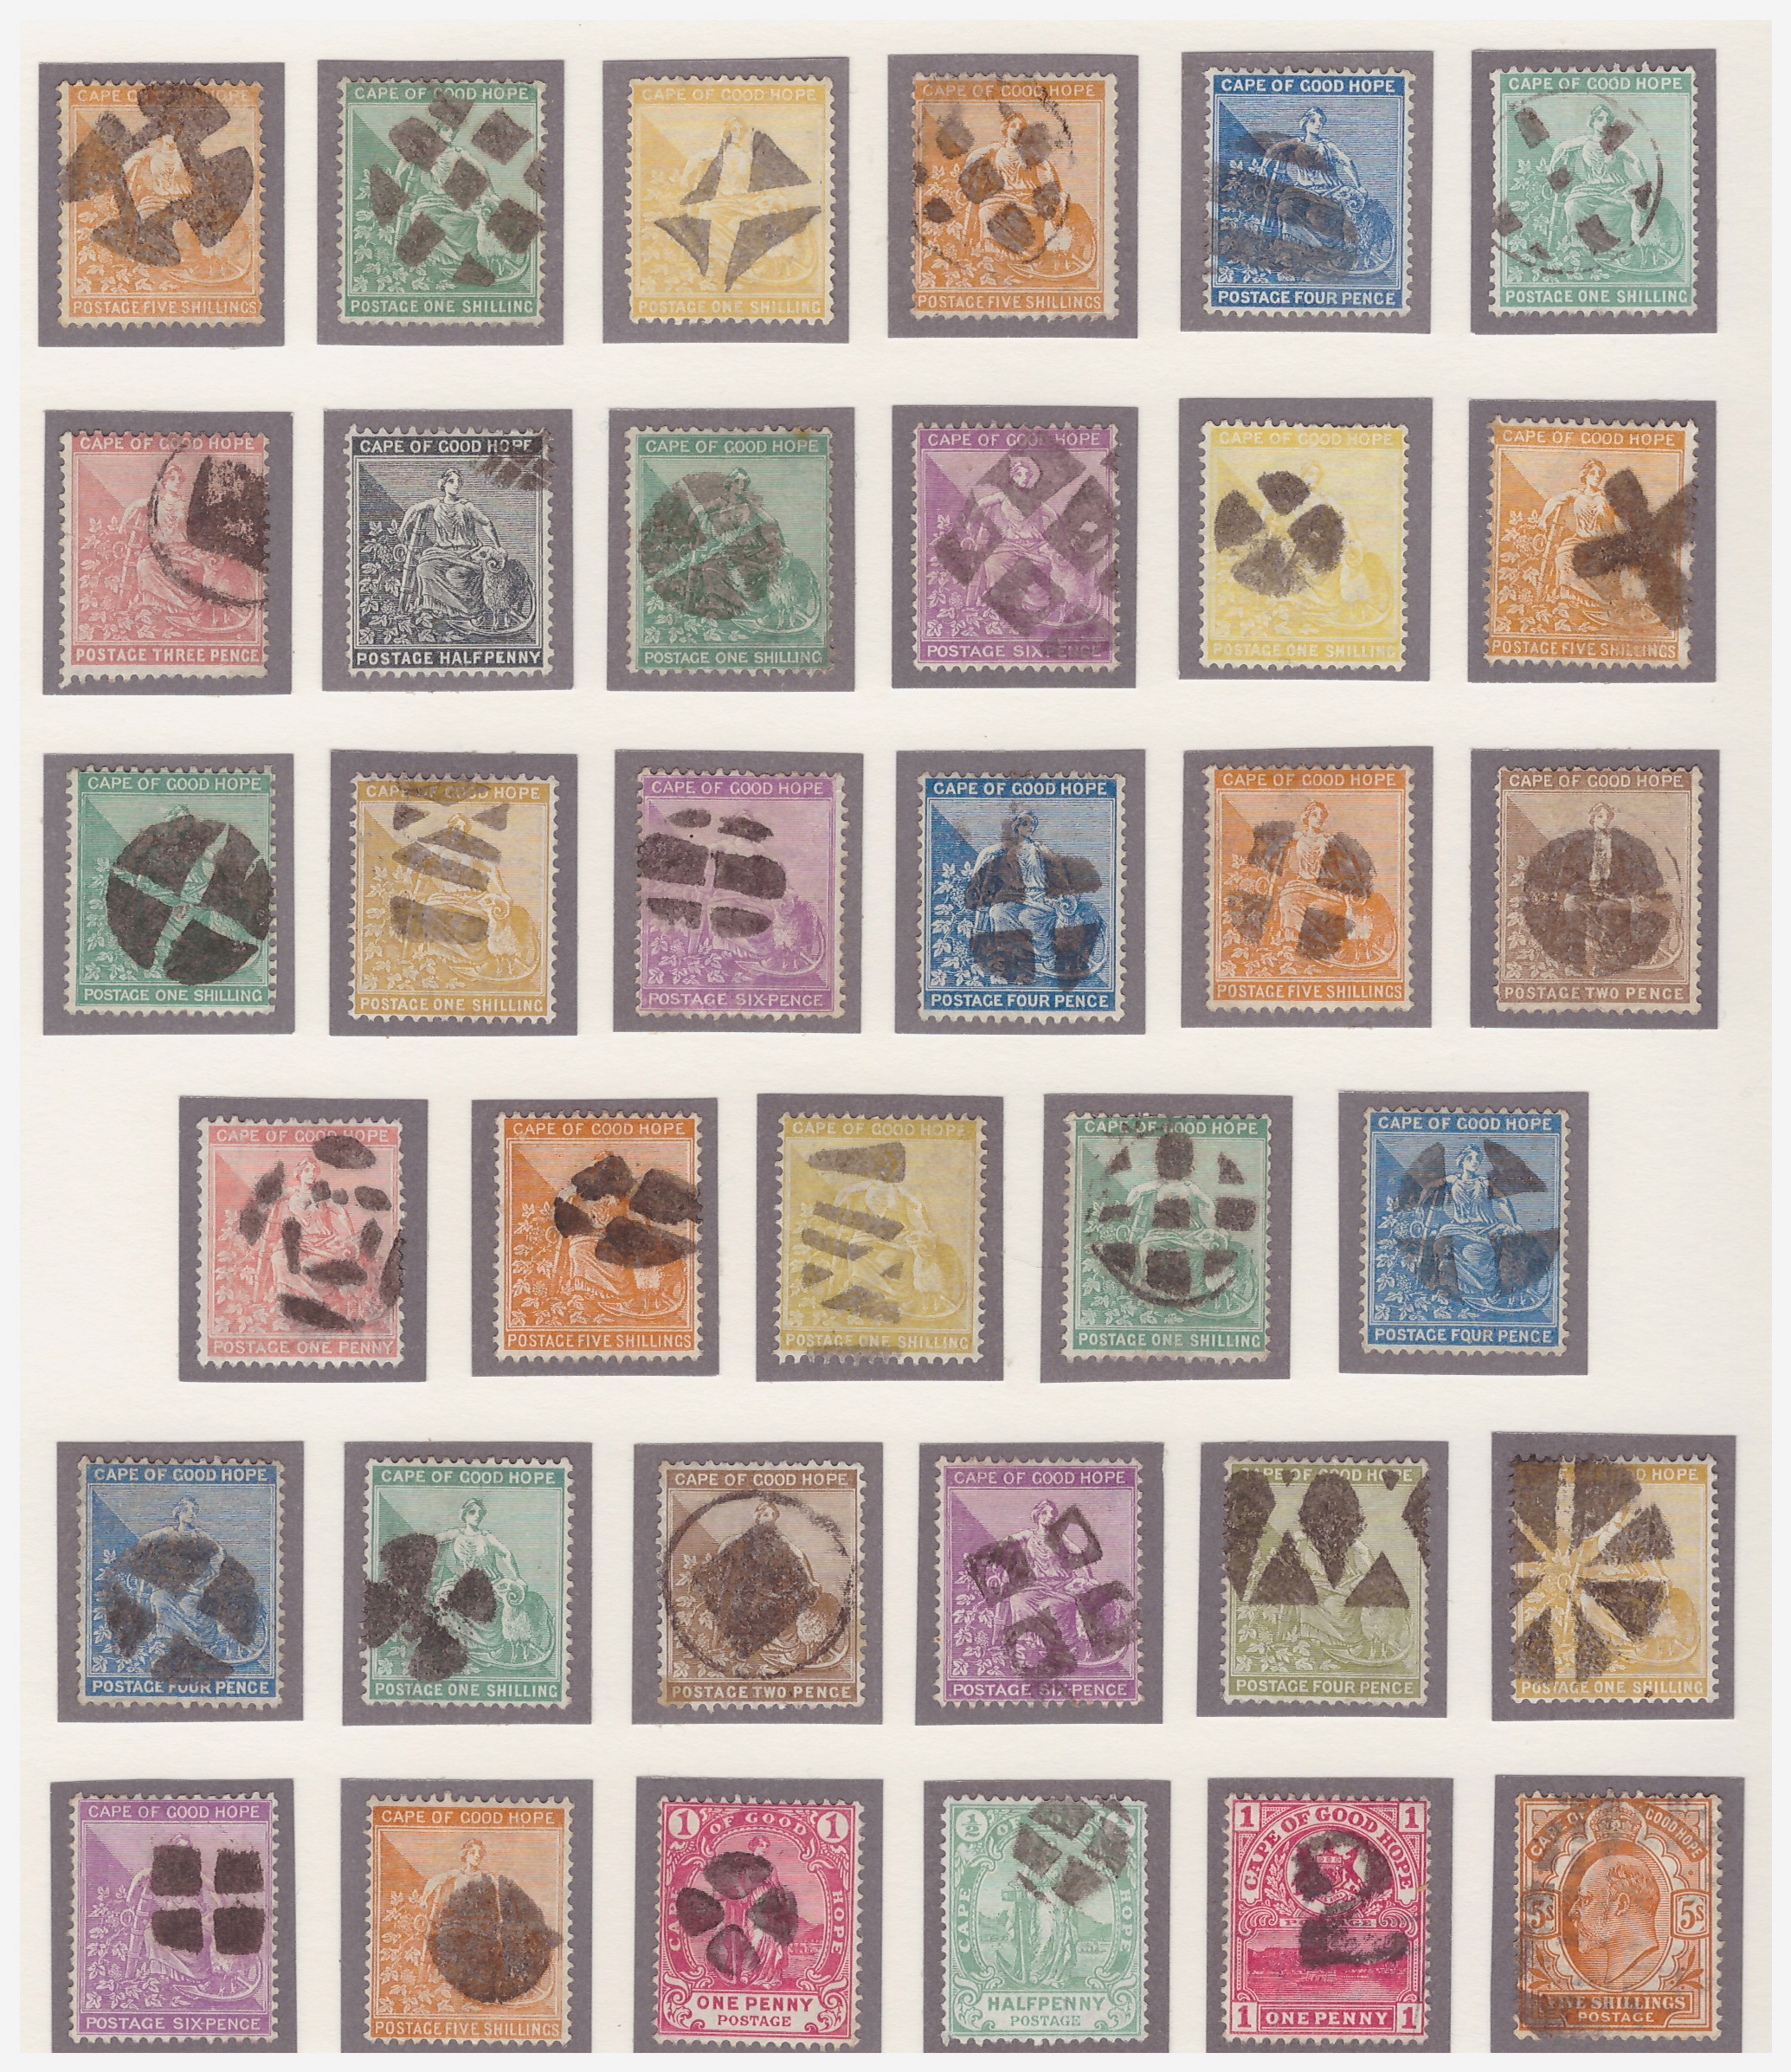
\includegraphics[width=1.0\textwidth]{../cape-of-good-hope/corks.jpg}
\end{figure*}

\clearpage


 
\ph[width = .80\textwidth]{../cape-of-good-hope/parcel-post/cork-on-cover.jpg}{
1899 (6th March), cover from the Transvaal, addressed to Holland and 
bearing a single$\frac{1}{2}$ on 1/- green surcharge (SG 198e) tied by Pretoria (6 Mar) datestamp. 
Also bearing, at upper left, a single Cape 1d carmine 
"Hope Standing"
 rectangle (SG 59a) tied by three strikes of a 
 CORK
 canceller. The reason for the addition of the Cape adhesive 
 is not clear. Backstamped Groningenen (25 Mar) arrival 
 datestamp. Clear BPA certificate (1998). Most unusual usage.
}
 

\ph[width = .80\textwidth]{../cape-of-good-hope/parcel-post/cork-on-cover-2.jpg}{
1895 CORK CANCEL PROVING COVER: GARDENS to MOSSEL BAY: Cover 
franked 1d Hope Standing superbly tied by complete cork cancel - 
shaped as multi-segmented retta style forming a circle. Front shows 
Gardens TO departure cds JU 19 with transit (Cape Town JU 19) and 
arrival mark (Mossel Bay JU 21) on reverse. Attractive, very rare. ...gckm/097	
Price: \$ 940
}
 

 

 
                  